% Template for Carleton problem sets
% Author: Andrew Gainer-Dewar, 20131
\documentclass[twoside]{article}
\usepackage{ccpset}
\usepackage{graphicx}

% The Latin Modern font is a modernized replacement for the classic
% Computer Modern. Feel free to replace this with a different font package.
\usepackage{lmodern}

\title{EE445L - Lab03 Report}
\author{Kevin Gilbert\\Gilberto Rodriguez}
\date{February 14, 2014}
\prof{Professor Bard}
\course{Lab: Monday/Wednesday 5-6:15}

\begin{document}
\maketitle{}

\section*{Objectives and Requirements Document}
 • Develop a graphics driver for the OLED that can plot lines and circles\\
• Design a hardware/software interf
ace for a keyboard or individual switches\\
• Design a hardware/software driver for generating a simple tone on a speaker\\
• Measure supply current necessary to run the embedded system\\
• Implement a digital alarm clock using periodic interrupts\\
\subsection{Requirements Document}

\subsubsection{Objectives}
The objectives of this project are to design, build and test an alarm clock. Educationally, students are learning how to design and test modular software and how to perform switch/keypad input in the background.
\subsubsection{Process} 
The project will be developed using the LM3S1968 board. The system will be built on a solderless breadboard and run on the usual USB power. The system will use external switches, one on board switch, and the on board speaker. There will be four hardware/software modules: 
\begin{enumerate}
\item switch/keypad input
\item time management
\item OLED graphics 
\item sound output
\end{enumerate}
The process will be to design and test each module independently from the other modules. After each
module is tested, the system will be built and tested.
\subsubsection{Roles and Responsibilities} 
\subsubsection{Interactions with Existing Systems} 
The system will use the LM3S1968 board, a solderless
breadboard, and be powered using the USB cable.
\subsubsection{Terminology} 
\begin{enumerate}
\item Power budget - estimate of the operation time of a battery-powered embedded system by dividing the enery storage by the average current requried to run the system
\item device driver - a collection of software routines that perform I/O functions
\item critical section - locations within a sofware module, which if an interrput were to occur at one of these locations, then an error could occur (e.g., data lost, corrupted data, program crash, etc)
\item latency - response time of the computer to external events
\item time jitter - undesired deviation from true periodicity of an assumed periodic signal in electronics and telecommunications, often in relation to a reference clock source
\item modular programming - a style of software development that divides the software problem into distinct and independent modules
\end{enumerate}
\subsubsection{Security} 
The system may include software from StellarisWare and from the book. No software written for this project may be transmitted, viewed, or communicated with any other EE445L student past, present, or future (other than the lab partner of course). It is the responsibility of the team to keep its EE445L lab solutions secure.
\subsection{Function Description}
\subsubsection{Functionality} 
The clock must be able to perform
five functions.
\begin{enumerate}
\item It will display hours, minutes, and seconds in
both graphical and numeric forms on the OLED. The graphical output will include the 12 numbers around a circle, the hour hand, the minute hand, and the second hand. The numerical output will be easy to read. 
\item It will allow the operator to set the current time using switches. 
\item It will allow the operator to set the alarm time including enabling/disabling alarms. 4) It will make a sound at the alarm time.
\item It will allow the operator to stop the sound.
\end{enumerate}
An LED heartbeat will show when the system is running.
\subsubsection{Prototypes} 
A prototype system running on the LM3S1968 board and solderless breadboard will be demonstrated. Progress will be judged by the preparation, demonstration, and lab report.
\subsubsection{Performance} 
The system will be judged by three qualitative measures. First, the software modules must be easy to understand and well-organized. Second, the clock display should be beautiful and effective in telling time. Third, the operation of setting the time and alarm should be simple and intuitive. The system should not have critical
sections. All shared global variables must be identified with documentation that a critical section does not exist. Backward jumps in the ISR should be avoided if possible. The interrupt service routine used to maintain time must complete in as short a time as possible. This means all OLED I/O occurs in the main program. The average current on the +5V power will be measured with and without the alarm sounding.
\subsubsection{Usability} 
There will be four switch inputs. In the main menu, the switches can be used to activate 
\begin{enumerate}
\item set time 
\item set alarm
\item turn on/off alarm
\item display mode.
\end{enumerate}
In set time and alarm modes, two switches add and subtract hours and the other two add and subtract minutes. After 10 seconds of inactivity the system reverts to the main menu. This functionality can be enabled by uncommenting a \emph{\#define} in SysTickInts.c in which we disabled this feature to allow debugging. The
display mode switch toggles between graphical and numeric displays. The switches will be debounced, so only one action occurs when the operator touches a switch once. The OLED display shows the time using graphical display typical of a standard on the wall clock. The 12
numbers, the minute hand, and the hour hand are large and easy to see. The clock can also display the time in numeric mode using numbers. The alarm sound is a simple square wave. The sound amplitude will be just loud enough for the TA to hear when within 3 feet.
\subsubsection{Safety} 
The alarm sound will be VERY quiet in order to respect
other people in the room during testing. Connecting or
disconnecting wires on the protoboard while power is applied may damage the board.
\subsection{Deliverables}
\subsubsection{Reports} 
A lab report described below is due by the due date listed in the syllabus. This report includes the final requirements document.
\subsubsection{Audits} 
The preparation is due at the beginning of the lab period on the date listed in the syllabus.
\subsubsection{Outcomes} 
There are three deliverables: preparation, demonstration, and report. 
\begin{pset}
  \problem{1}
    \textit{You can either call the start and end critical sections functions from Startup.s to disable interrupts, or remove global dependencies.}
  \problem{2}
	How long does it take to update the OLED with a new time?\\
    \textit{The ISR takes a few clock cycles to update the time variables. Drawing to the OLED takes considerably more time, and is not located in the ISR. The buffer is roughly 6200 bytes in size, and must be transfered to the OLED.}
  \problem{3}
  	What would be the disadvantage of updating the OLED in the background ISR?\\
    \textit{Updating the OLED in the background ISR would increase the time in the ISR and miss other interrputs that would fire such as a timer interrput or button interrupt.}
   \problem{4}
	Did you use a OLED clear function? If so, how could you have redesigned the OLED update to run much faster?\\
    \textit{We did use an OLED clear function. There was a lot of space on the borders that remained the same. Selectively clearing portions would have been more efficient.}
   \problem{5}
	Assuming the system were battery powered, list three ways you could have saved power.\\
    \textit{We could have slowed down the PLL to conserve power, as well as utilize hibernate mode between interrupts and operations. We could also use lower power external speakers as the internal ones seem to use a lot of power. }

\end{pset}
\section*{Measurements}
-> RMS voltage 3.31, 4.94.
-> Current 56mA without speaker, 0.58mA-270mA

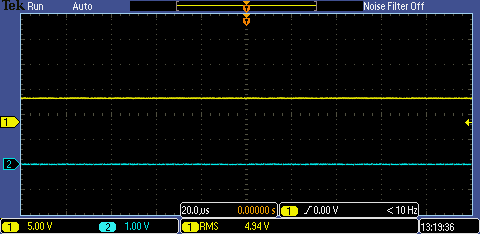
\includegraphics[width=1\textwidth]{TEK00000}
\centerline{\textit{Figure A: 5V vs time}}
\vskip 0.25in
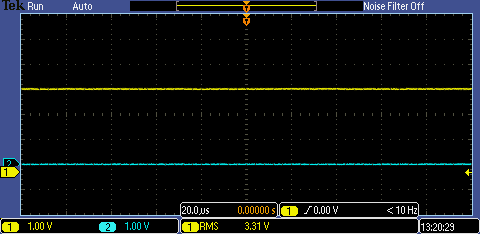
\includegraphics[width=1\textwidth]{TEK00001}
\centerline{\textit{Figure B: 3.3V vs time}}
\vskip 0.25in
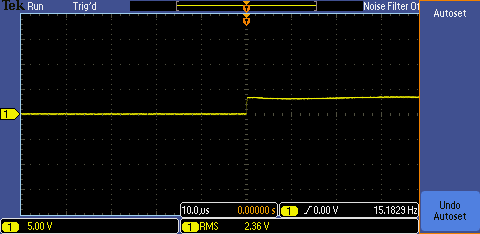
\includegraphics[width=1\textwidth]{TEK00002}
\centerline{\textit{Figure C: Voltage when alarm is on}}
\vskip 0.25in
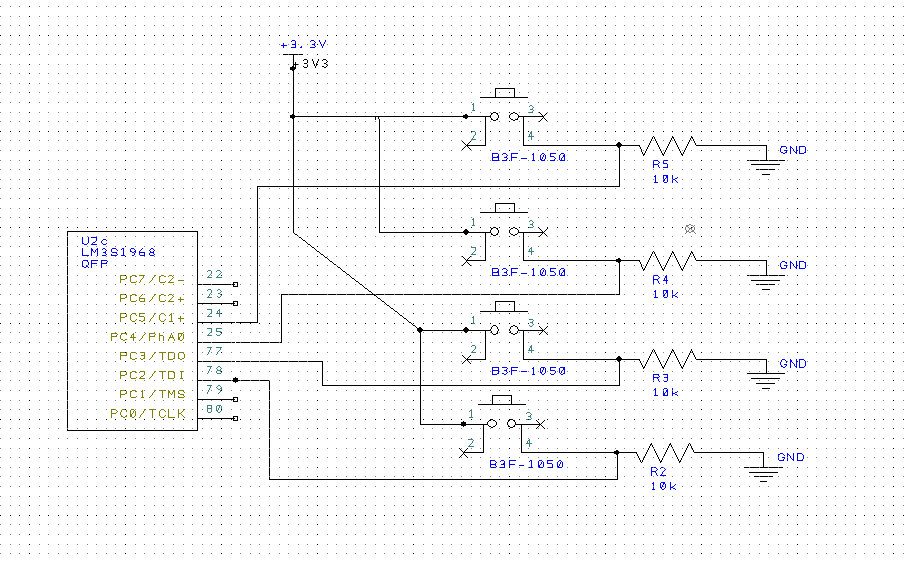
\includegraphics[width=1\textwidth]{Circuit}



\end{document}